%background
\section{Parameters}
The ``input'' to a program is a set of parameters, named variables that represent specific groups of data points. How those parameters are generated, and what literal form they take, effects the outcome of the program. Large programs with larger inputs may benefit from having their input parameter data sets generated by statistical distributions.

I was inspired to create this tool by testing a project I helped build in my software engineering class, which took in the records of each student in a class of 40 students, describing things like their skills in certain technologies and their available free times during the week. This project made a fairly sophisticated decision about how to form optimal groups of students to work in teams, ensuring that each group has complementary skills and overlapping free times. During testing, it is important to consider bizarre scenarios, like what should happen when no student has any free time at all, or when half the class can only meet early in the week and the other half can only meet late in the week. If the tool can gracefully handle situations like this, it gives me as a tester confirmation that the software functions the way I expect it to. These ``edge case'' scenarios scarcely happen in real life. But it is important to test them because they very well might happen in real-life, and in a production environment the software needs to be able to handle it. Moreover, software that can handle the variety of situations indicates that it has very few bugs, if any.

These parameters can follow certain trends that can be mimicked by repeated trials of statistical distributions. The input to this program is merely an Excel csv file of a record table, such that every row is a student's entry and every column is all the entries for a certain parameter that really effects the outcome of the program. Figure \ref{fig:teamfile} shows the CSV file of the literal input into the Team Building program. The software takes in the filename, opens the file, and parses the data. Each row is a student, and each column is a parameter, such as free time availability on Monday or self-rated HTML experience level.

\begin{figure}
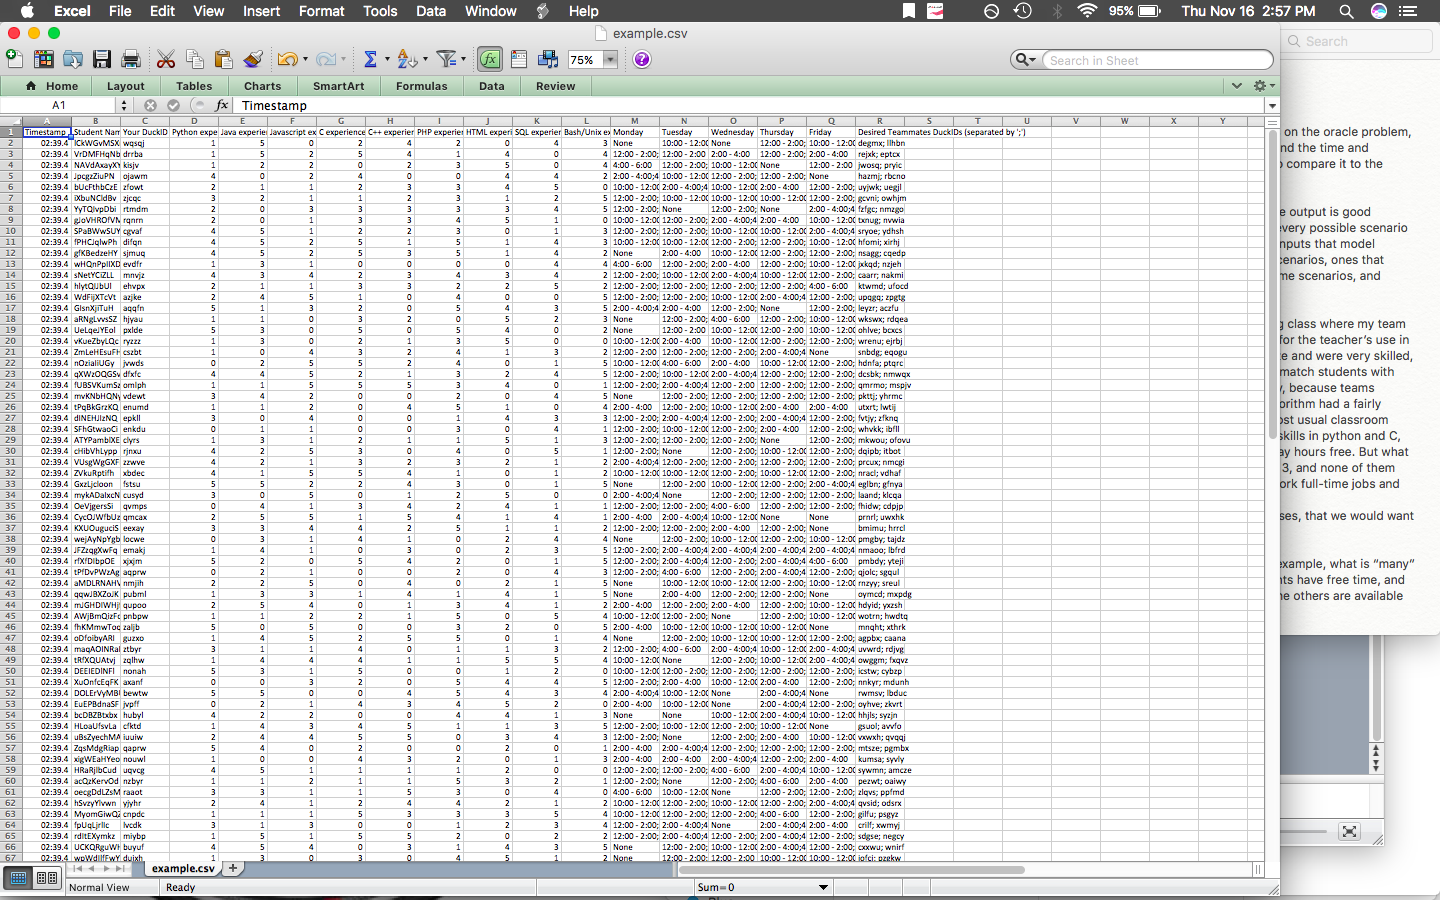
\includegraphics[scale=0.3]{team-file.png}
\caption{A CSV file of a test case input into the Team Builder program}
\label{fig:teamfile}
\end{figure}

\section{Pairwise Testing}
GenPairs is a pairwise testing tool~\cite{Gen:Pairs} that creates symbolic test vectors that describe what each test case should generally look like, using English adjectives to describe what the input should be. Pairwise testing rests on the hypothesis that a majority of faults in a program are a result of combinations of parameters that work with one another to create or amplify a problem. Creating the minimum number of test cases that satisfactorily describe all combinations of possible parameters gives adequate code coverage. The success of finding all faults increase with greater numbers of combinations of parameters; that is to say that all combinations of four parameters will find more faults than all combinations of three. However, pairwise testing finds all combinations of two parameters and is sufficient for code coverage while still reducing the time, and therefore cost, of creating or running potentially hundreds of other test cases. This is even more effective when the total number of parameters is also somewhat low. Combining only two parameters is a matter of convenience and time, since more test cases require more time to create and to execute.

While translating a symbolic test vector to concrete data may present a challenge, it is extremely valuable in reducing the uncertainty of knowing what sort of trend the input test data follows. Say, for example, a tester needs to generate a concrete point for this test vector (Table \ref{table:testv})

\begin{table}[h!]
\centering
\begin{tabular}{@{} *5l @{}}    \toprule
\emph{Item Purchased} & \emph{Price} & \emph{Delivery Method}  \\\midrule
Large Item & Expensive & Ultrafast \\\bottomrule
 \hline
\end{tabular}
\caption{Single Symbolic Test Vector}
\label{table:testv}
\end{table}

She knows that some test case will send a large item by ultrafast means. In our generation of concrete data (described in the next section) in this test vector, she might come across the test case in Table \ref{table:conctc}

\begin{table}[h!]
\centering
\begin{tabular}{@{} *5l @{}}    \toprule
Motorboat & 18700.00 & Jet Airplane \\\bottomrule
 \hline
\end{tabular}
\caption{Single Concrete Test Case}
\label{table:conctc}
\end{table}

The interaction of these two parameters, a very large object sent by ultrafast means, ought to trigger a bug in the system, because perhaps her company does not have that capability. If this situation is not handled correctly in the software, the user of the software, the customer, will be misled about the quality of their shipping network. This example is very trivial, but it exemplifies the problem well, and shows how pairwise testing methods can bring this awareness to the tester and developer and help them improve their software. Now imagine a much longer and complicated test vector in a very advanced version of the company’s ecommerce website; maybe now it has millions of possible item categories and hundreds of shipping methods and can also handle coupon codes and student discounts and special offerings: many more parameters to consider. It is helpful to know that the test vector was created from a description including Large Item - Expensive - Ultrafast. The symbolic test vector describes the input well enough for the tester to understand and use common sense to predict what the output ought to be. Then if she tests that test case and finds that the customer receives a message that sending a boat through lightning speed mail is impossible, she gains more confidence that her program works correctly.

The pairwise testing tool is designed such that the tester describes all the possibilities for what each parameter could possibly be, and then the tool generates all the test vectors that describe what the parameter ends up becoming. When using this tool, testers should list every kind of statistical distribution that they would be interested in seeing, or what makes sense in the context of their program. This is so important because it makes GenSequence a more applicable tool for database-driven applications. If a tester would benefit from giving meaning to the data trend, they can benefit from using the GenSequence framework. This is the semantic sense that is often missing in testing database programs.

Most importantly, Pairwise testing satisfies the need to test ``outlier'' cases. The very function of pairwise testing ensures that a combination of classifications of parameters occurs at least once in the test suite. This is a test case that the tester might have otherwise forgotten or overlooked. It guarantees robust testing.

\section{Context-Free Grammars}
We can use the ideas of context-free grammar derivations to generate concrete test data. We call this feature Makogram, a tool implemented in the Python templating tool Mako~\cite{Mako:Template}. Say a test case has the following production rule:

\begin{grammar}
<Case> ::= <Item> <Price> <Delivery Method>
\end{grammar}

What constitutes an item? Item might have a production rule

\begin{grammar}
<Item> ::= `Ship' | `Book' | `Loaf'
\end{grammar}

The grammar tool used is constructed such that a non-terminal can be the result of a function, and that result can be a randomly generated data point. For example,

\begin{grammar}
<Price> ::= fun \{ random_choice(8,15) \} ( )
\end{grammar}

Meaning that the data point for the Price parameter would be some number chosen at equal randomness from any number between 8 and 15.

A terminal symbol can be written to be the returned result of a much more sophisticated function - one perhaps that returns a Gaussian distribution of data points. For example, consider an earthquake modeling program, which takes a set of data points for its magnitudes parameter, and it can have all sort of descriptions attached to it: Gaussian, uniform, cardioid, etc. All of these descriptions will occur somewhere in a test vector, so each is mapped to the corresponding function. When the magnitudes parameter is set to be generated from a bell-curve distribution, the bell-curve random generator will generate that set of points.

Generating good test data for actual magnitudes of an earthquake must be based on the knowledge that a magnitude cannot be negative or greater than 10.0. This is the limit of the program. It cannot make logical guesses about the natural language of the parameter. But the tool is written to minimize the number of times the tester must identify this constraint –- just once, in the beginning.

Moreover, the power of grammars makes creating the data very easy. GenSequence provides support for the \textit{grammar} of the output csv files, which can be thought of as a template describing the ``language'' of a csv file. A derivation is a series of rule substitutions that eventually ends with a string. This ``string'' belongs to the language described by the grammar, and this string \textit{is} the test data that is usable for testers because the production rules gave functional data points. Makogram was constructed not just to limit the number of substitutions but to reach exactly the desired number. So if a tester asks for 30 examples (30 rows of data), Makogram will hand back exactly 30 rows.

\section{Law of Large Numbers}
The Law of Large Numbers states that the actual outcomes will approach the expected outcomes as the sample size increases to infinity . One canonical example is a series of coin flips, with an equal probability of flipping heads as tails. It is expected that exactly 50\% of the samples will be heads and 50\% tails. In a sample size of only one hundred flips, the percentage of heads to tails may only be 46.0\% - 54.0\%, but a sample size of ten thousand would come far closer to an even 50-50 split, possibly 50.37\% - 49.63\%. 

This principle applies to all kinds of probability distribution types, not just coin flip probability. Students’ grades tend to figure towards a bell-curve distribution, but a graph of 50 students’ grades will look more misshapen than a graph of thousands of students’ grades. Moreover, the principle applies to many programming languages’ utilities that support randomness. The Python language contains a built-in module called random which provides a variety of generators for all flavors of probability distribution. Individual points are generated according to a particular distribution, and the generation of a large enough sample size is guaranteed to follow the expected trend.

How large is large? Bernoulli proved that the actual outcome of a simulation would approach the expected outcome as the sample size grows to infinity. So in general, the greater the sample size the more accurate the results.

If the use case arrives on the order of hundreds of data points, a default sampling size on the order of ten thousand randomly generated data points should suffice. Because the initially generated set of points is far too many, I have devised a scheme to reduce the sample set to the appropriate size while still encapsulating the distributions guaranteed by the Law of Large Numbers. For each parameter, I generate the too-large sample size, sort it in increasing order, and selectively choose every nth point to include in the reduced set of points, such that the size of the reduced set is the desired number –-  however many the test case needs.\footnote{Given the statements of the previous section, some clarification is in order. Context-free grammars would imply that the random function would be called upon every derivation of a data point. But since the number of derivations is limited, that would mean that the number of function calls would be minimized, which would not produce the desired distribution. GenSequence declares the grammar, and then uses what I call a Parm object to create a large sample size and reduce it down into a small pool. When a derivation of the grammar is instantiated, it calls upon the pool, which yields singular points.}

I have yet to rigorously prove this selection scheme, but I hypothesize that it suffices for now, and does indeed capture the essence of the Law of Large Numbers. Pictorial representations show that this paradigm is not perfect, but is certainly far better than choosing exactly the desired number of points. Visibly a sample size of 300 systematically chosen from a large set follows the curve of 10,000 points much more closely than 100 initial points.

\begin{figure}[H]
\centering
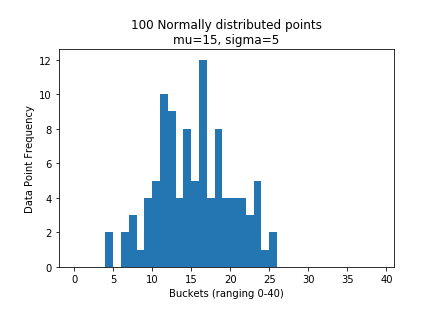
\includegraphics[scale=0.7]{law1.png}
\caption{Histogram of point values generated by normal distribution - sample size 100}
\label{fig:law1}
\end{figure}

\begin{figure}[H]
\centering
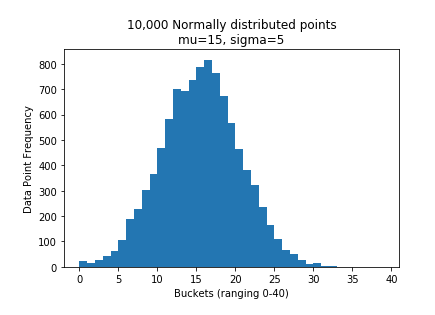
\includegraphics[scale=0.7]{law2.png}
\caption{Histogram of point values generated by normal distribution - sample size 10,000}
\label{fig:law2}
\end{figure}

\begin{figure}[H]
\centering
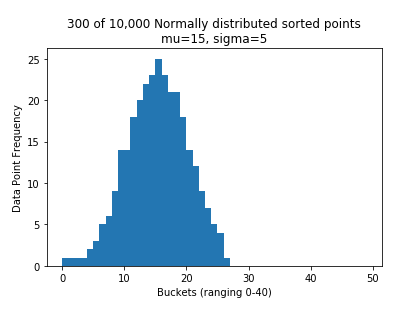
\includegraphics[scale=0.7]{law3.png}
\caption{Histogram of point values generated by normal distribution and reduced to sample size of 300}
\label{fig:law3}
\end{figure}


\section{Cardioids}

In some testing situations, it may be useful to consider the relationship between two parameters, a relationship that mimics real life. For example, a physics-modeling simulation might have a loose property that larger objects move slower than smaller objects. These two parameters, size and velocity, are interdependent.

A Cardioid\footnote{The name cardioid was chosen for its polarity. Its figure encompasses an area such that a majority of the space (about 90\%) sits on one side of an axis and a small section (about 10\%) sits on the other.} object acts as a two-column parameter. The end user specifies the relationship between the two sub-parameters by providing descriptions of what data point range pairings are preferred (called favorites) and what data point range pairings should only occur infrequently (called outliers or non-favorites). The data generation step will look at these descriptions and generate the data point pairings such that 90\% of the samples are favorites and 10\% are outliers. For example, the tester will specify favorites for the cardioid relationship between size and velocity: large and slow, medium and medium, and small and fast. Non-favorites are outlying particles: small and slow, and large and fast.

The cardioid relationship spanning two parameters occurs only if the tester specifies it as a possibility in the test vector creation step. There are certainly situations where it does not make semantic sense to use cardioid relationships, and in that case, cardioids are not required for test data generation. On the other side, statistical distributions may not make semantic sense because they do not raise \textit{every} test case one wants to check. Cardioids allow the user to include their own test data generation constraints if statistical randomness does not quite suffice, and allows for tests that maintain or exaggerate realistic sense. Again this is a tool that helps testers identify and execute edge cases.

\section{Preprocessing}

An important arm of the automation pipeline is developing a baby-sized language, a little language~\cite{Bentley:1986:PP:600875}, that is easy to write yet fully describes everything a tester wants out of this tool. Then a preprocessor can read this language and generate the code that, when executed, will create the data. Writing the data-generating code itself is complex enough that it limits automation, and building a machine that performs this step systematically significantly increases ease of use. I have fully developed the language into basic syntax and grammar rules, which the tester can then write in a .prm file.

I have also constructed a simple preprocessor to parse this information. It is very lightweight in that it compiles quickly, but does not have advanced error handling or give helpful compiler errors. The current iteration implements Ply (Python Lex-Yacc)~\cite{PythonLexYacc}. Ply works in two general steps. First it reads the input and identifies characters or words into tokens –- essentially describing the type of each word or character. This is the lexing, or ``tokenizing'', step. Next, the parsing step, parses the tokens altogether by identifying the grammar rules that combine them. Once the information has been identified as a derivation of a grammar rule, it is then available for interpretation. The preprocessor does not yet use Ply to read the entire .prm file, and mostly uses Python file-processing techniques, but the language is simple enough that I had little difficulty rendering the information into the data generator. For an MVP this tactic suffices.
